% !TEX encoding = UTF-8 Unicode
% !TEX TS-program = LuaLaTeX
% !TEX root = ../memoire.tex
% !TEX spellcheck = fr-FR

%************************************************
\chapter{Arbres et forêts}
\label{chap:quatre}
%************************************************

\section{Arbres de décision}

\todo{Trop "inspiré" de Louppe.}

La performance pure des méthodes statistiques a toujours été l'un des principaux moteurs de la recherche dans le domaine, mais cela n'est pas le seul critère de la qualité d'un modèle. En effet, l'interprétabilité d'un modèle est dans beaucoup de domaines aussi, si ce n'est plus, important que la performance du modèle. Parmi ces modèles explicatifs, l'un sort du lot par sa combinaison de bonnes performances et facilité de compréhension: les arbres de décision. Nous suivrons les notations et définitions de \citet{Louppe2014}, et renvoyons à sa thèse pour un aperçu exhaustif de la littérature existante ainsi qu'une analyse de l'implémentation et la complexité algorithmique des arbres et forêts aléatoires, ce chapitre n'a pas donc vocation a apporter un point de vu original.
Historiquement introduit par Morgan et Sonquist en 1963 la version moderne de ces arbres a été introduite indépendamment par Breiman, Friedman et Quinlan. Plus précisément c'est le modèle \ac{cart} de \citet{Breiman1984a} qui introduit de façon rigoureuse et unifiée la théorie des arbres de décision.
Avant même d'en étudier leurs caractéristiques, il est possible de donner plusieurs raisons expliquant la popularité des arbres de décision
\begin{itemize}
    \item Ils sont non-paramétriques.
    \item Ils peuvent traiter les données hétérogènes (mélange de variables qualitatives et quantitatives) ainsi que les données manquantes.
    \item Ils effectuent automatiquement une sélection des variables et sont donc en partie résistants aux variables inutiles ou bruitées.
    \item Ils sont résistants aux outliers ou erreurs d'étiquetage.
    \item Ils sont faciles d'interprétation.
\end{itemize}

\subsection{Structure}

De la façon la plus générale, on peut voir un arbre de décision comme une partition récursive de l'espace ce qui est tout particulièrement adapté aux problèmes de classification. En effet si $\mathcal{Y} = \{c_1, \dotsc, c_j \}$\label{ntn:c_k} est l'espace des classes, alors on peut voir notre problème de classification supervisée sur $\Omega$ comme une partition 
\begin{equation*}
    \Omega = \Omega_{c_1} \cup \dotsc \cup \Omega_{c_j}    
\end{equation*}
avec $\Omega_{c_k}$ l'ensemble des individus de classe $c_k$. On peut donc voir notre classifieur $\varphi$ comme une partition de l'espace puisqu'il définit une approximation $\hat{Y}$ de $Y$, à l'exception que cette partition se fait sur $\mathcal{X}$ au lieu de $\Omega$ directement. On a alors:
\begin{equation*}
    \mathcal{X} = \mathcal{X}^{\varphi}_{c_1} \cup \dotsc \cup \mathcal{X}^{\varphi}_{c_j}
\end{equation*}
où $\mathcal{X}^{\varphi}_{c_k}$ est l'ensemble des $x \in \mathcal{X}$ tels que $\varphi (x) = c_k$. Notre problème d'apprentissage peut alors se réécrire comme un problème d'approximation de la partition optimale de Bayes:
\begin{equation*}
    \mathcal{X} = \mathcal{X}^{\varphi_B}_{c_1} \cup \dotsc \cup \mathcal{X}^{\varphi_B}_{c_j}
\end{equation*}

Nous pouvons donc maintenant créer nos arbres comme des partitions récursives de l'espace.

\begin{definition}[Arbre enraciné]
    Un arbre enraciné est un graphe acyclique orienté $G=(V,E)$ où l'un des nœuds est désigné comme racine et toutes les arrêtes fuient la racine.
\end{definition}

\begin{definition}[Nœuds]
    S’il existe une arrête de $t_1$ vers $t_2$ alors $t_1$ est appelé nœud père de $t_2$ et $t_2$ nœud fils de $t_1$. 
\end{definition}

\begin{definition}
    Un nœud d'un arbre enraciné est dit interne s’il possède au moins un fils et terminal (ou feuille) sinon.
\end{definition}

\begin{definition}
    Un arbre binaire est un arbre enraciné où chaque nœud interne possède exactement $2$ fils: le fils gauche et le fils droit notés à partir d'ici respectivement $t_L$ et $t_R$.
\end{definition}

Dans ces conditions, un \emph{arbre de décision} est un classifieur $\varphi : \mathcal{X} \rightarrow \mathcal{Y}$ représenté par un arbre enraciné où chaque nœud $t$ représente un sous-espace $\mathcal{X}_t \subseteq \mathcal{X}$ avec la racine $t_0$ représentant $\mathcal{X}$ tout entier. Les fils $t_i, \dotsc, t_j$ de $t$ représentent alors une partition disjointe de $\mathcal{X}_t$. Chaque feuille est alors étiquetée avec $\hat{y}_t \in \mathcal{Y}$, la meilleure approximation possible de $y$. Si $\mathcal{Y} = \{c_1,\dotsc,c_j\}$ alors l'arbre est dit de classification, si $\mathcal{Y} = \mathbb{R}$ il est dit de régression, ce ne sont pas les seuls types d'arbres possibles et l'on peut notamment citer les arbres de quantiles \citep{Meinshausen2006}, de densités \citep{Ram2011} ou de survie \citep{Ishwaran2008}. Alors $\varphi(x)$ est l'étiquette de la feuille atteinte à partir de $t_0$ en suivant les règles de coupure. Le choix de représenter un problème de classification par un graphe acyclique est tout à fait raisonnable. En effet, on cherche à modéliser un système complexe par les interactions entre les différentes variables aléatoires qui le composent, ce qui correspond exactement au cadre général plus vaste des \emph{modèles graphiques}. Néanmoins en restreignant le type de graphe considéré on se ramène à un problème de partitionnement bien plus facile à étudier que ce soit de manière théorique ou dans la résolution pratique.

Le choix de représenter le problème sous la forme d'arbres est arbitraire et ne sert qu'à rendre les calculs plus faciles, il est tout à fait envisageable de détendre les restrictions sur la forme du graphe et autoriser par exemple plusieurs ancêtres. Les performances peuvent ainsi être améliorées au détriment de la facilité de calcul \citep{Shotton2013a}.

\begin{figure}[htbp]
    \centering
    \begin{subfigure}[b]{.45\textwidth}
    \centering    
    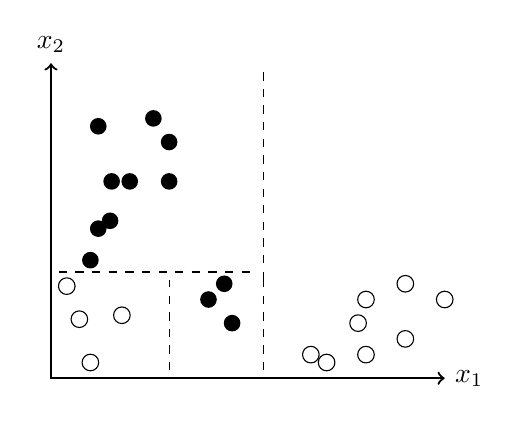
\begin{tikzpicture}
    % Draw axes
    \draw [<->,thick] (0,4) node (yaxis) [above] {$x_2$}
          |- (5,0) node (xaxis) [right] {$x_1$};
    % Draw line
    \draw[dashed] (2.7,0.1) -- (2.7,1.25);
    \draw[dashed] (2.7,1.25) -- (2.7,3.9);
    \draw[dashed] (0.1,1.35) -- (2.6,1.35);
    \draw[dashed] (1.5,0.1) -- (1.5,1.25);
    % Draw negative dots
    \fill[black] (0.5,1.5)   circle (3pt);
    \fill[black] (1.5,2.5)   circle (3pt);
    \fill[black] (1,2.5)     circle (3pt);
    \fill[black] (0.75,2)    circle (3pt);
    \fill[black] (0.6,1.9)   circle (3pt);
    \fill[black] (0.77, 2.5) circle (3pt);
    \fill[black] (1.5,3)     circle (3pt);
    \fill[black] (1.3,3.3)   circle (3pt);
    \fill[black] (0.6,3.2)   circle (3pt);
    \fill[black]   (2.2,1.2)   circle (3pt);
    \fill[black]   (2,1)   circle (3pt);
    \fill[black]   (2.3,0.7)   circle (3pt);
    % Draw positive dots
    \draw[black] (0.2,1.17)     circle (3pt);
    \draw[black] (0.5,0.2)     circle (3pt);
    \draw[black] (0.36,0.75)     circle (3pt);
    \draw[black] (0.9,0.8)     circle (3pt);
  
    \draw[black] (4,1)     circle (3pt); 
    \draw[black] (3.3,.3)  circle (3pt); 
    \draw[black] (4.5,1.2) circle (3pt); 
    \draw[black] (4.5,.5)  circle (3pt); 
    \draw[black] (3.9,.7)  circle (3pt); 
    \draw[black] (5,1)     circle (3pt); 
    \draw[black] (3.5,.2)  circle (3pt); 
    \draw[black] (4,.3)    circle (3pt); 
    \end{tikzpicture}
    \end{subfigure}
    ~
    \begin{subfigure}[b]{.45\textwidth}
    \centering
        \begin{forest}
        [$x_1 \leq 2.7$
            [$x_2 \leq 1.35$
                    [$x_1 \leq 1.5$
                        [,circle, draw]
                        [,circle, fill]
                    ]
                [,circle, fill]
            ]
            [,circle, draw]
        ]       
    \end{forest}
    \end{subfigure}
    \caption{Équivalence entre la partition du plan et un arbre de décision binaire}
\end{figure}

\subsection{Critère d'impureté}

Apprendre un arbre de décision revient alors à déterminer la plus petite des partitions la plus proche de la partition engendrée par $Y$ sur $\mathcal{X}$, ce problème est en réalité NP-complet et trouver la meilleure approximation est impossible en un temps raisonnable. Il est donc nécessaire de développer une heuristique permettant de construire l'arbre par induction en maximisant une fonction "objectif" assurant de faire un choix judicieux à chaque étape. Ainsi \citet{Breiman1984a} définissent une notion de mesure d'\emph{impureté} $i(t)$ qui évalue la qualité de la partition courante en $t$. Dans ce cadre, plus $i(t)$ est petit, plus le nœud est \emph{pur} et meilleure est la prédiction $\hat{y}_t (x)$, où $(x,y) \in \mathcal{L}_t$ avec
\begin{equation*}
    \mathcal{L}_t = \left \{ (x,y) \in \mathcal{L} \mid x \in \mathcal{X}_t \right\}    
\end{equation*}
et $\mathcal{X}_t$ le sous-ensemble de l'espace représenté par le nœud $t$ (donc $\mathcal{X}_{t'} \subset \mathcal{X}_t$ si $t'$ est un descendant de $t$ et $\mathcal{X} = \bigcup \mathcal{X}_t$).

On obtient ainsi tout naturellement un algorithme glouton de construction de l'arbre: en partant d'une racine représentant l'ensemble d'apprentissages tout entier (et donc l'espace tout entier) chaque itération divise la population du nœud courant de façon à minimiser l'impureté des nouveaux nœuds, l'algorithme s'arrête lorsque l'impureté ne peut plus être réduite.
Définissons alors la diminution de l'impureté pour une coupure binaire $s$ en $t$:

\begin{definition}
    La \emph{réduction d'impureté pondérée} d'une partition binaire $s \in \mathcal{Q}$ divisant $t$ en $t_L$ et $t_R$ est:
    \begin{equation*}
        \Delta i(s,t) = i(t) - p_L i(t_L) - p_R i(t_R)
    \end{equation*}
    où $p_L$ (resp. $p_R$) est le rapport $\frac{N_{t_L}}{N_t}$ (resp. $\frac{N_{t_R}}{N_t}$) d'échantillons d'apprentissage de $\mathcal{L}_t$ allant dans $t_L$ (resp. $t_R$) avec $N_t = \vert \mathcal{L}_t \vert$
\end{definition}

\subsubsection{Classification}

Dans le cas de la classification, le rôle de l'arbre est la minimisation de l'erreur de généralisation. Il peut donc sembler naturel de prendre pour $i(t)$ l'estimation locale de la certitude de classification en $t$.

\begin{definition}
    Dans le cas de la classification, l'\emph{impureté} $i_R (t)$ basée sur l'estimation locale de la certitude de classification définie sur la perte $0$-$1$ est:
    \begin{equation*}
        i_R (t) = 1 - p(\hat{y}_t \mid t ) = 1 - \max_{c \in \mathcal{Y}} p(c\mid t)
    \end{equation*}
\end{definition}
Ce choix est naturel puisqu’il revient à choisir la coupure qui minimise l'erreur d'apprentissage. Néanmoins cette notion d'impureté a plusieurs défauts:
\begin{enumerate}
    \item $\Delta i(s,t)$ vaut $0$ pour toutes les coupures pour lesquelles tous les fils gardent la même classe majoritaire, c'est-à-dire si $y_t = y_{t_L} = y_{t_R}$. Toutes les coupures sont alors considérées comme aussi bonnes.
    \item Il y a peu d'impact de la distribution a posteriori des classes $p(y\mid t_L)$ et $p(y\mid t_R)$.
\end{enumerate}
Ces défauts sont principalement dus au processus de création de l'arbre: puisque l'arbre est construit de manière gloutonne, il faudrait que notre notion d'impureté prenne en compte les possibilités de réduction future de l'impureté dans les étapes suivantes. Pour éviter les défauts de $i_R (t)$ le choix de $i(t)$ doit être fait de telle sorte que celui-ci décroît au fur et à mesure que les nœuds $t$ deviennent plus homogènes. Dans l'algorithme \ac{cart}, \citet{Breiman1984a} identifient une famille de fonctions d'impureté $i(t)$ qui répond à ce critère:
\begin{theoreme}
\label{impurete}
    Soit $\Phi (p_1,\dotsc,p_J)$ une fonction strictement concave définie sur $0 \leq p_k \leq 1$, pour $k=1,\dotsc,J$ et $\sum_{k=1}^J p_k = 1$ telle que:
    \begin{itemize}
        \item $\Phi (1,\dotsc,0) = \Phi (0,1,\dotsc,0) = \dots = \Phi ( 0,\dotsc,1)$ soit minimale
        \item $\Phi \left(\frac{1}{J},\dotsc,\frac{1}{J} \right)$ soit maximale
    \end{itemize}
    Alors pour $i(t) := \Phi \left( p(c_1 \mid t), \dotsc, p(c_J \mid t) \right)$ et pour n'importe lequel $s$,
    \begin{equation*}
        \Delta i(s,t) \geq 0
    \end{equation*}
    avec égalité si et seulement si $p(c_k \mid t_L) = p(c_k \mid t_R) = p(c_k \mid t)$ pour $k=1,\dotsc,J$
\end{theoreme}
Les critères d'impuretés les plus courants dans le cas des arbres de classifications sont l'entropie de Shannon et l'indice de Gini:
\begin{definition}
    La fonction d'impureté $i_H (t)$ basée sur l'entropie de Shannon \citep{Shannon1957} est:
    \begin{equation*}
        i_H (t) = - \frac{1}{2} \sum_{k=1}^J p(c_k \mid t) \log_2 \left( p(c_k \mid t ) \right)
    \end{equation*}
\end{definition}
\begin{definition}
    La fonction d'impureté $i_G (t)$ basée sur l'indice de Gini est:
    \begin{equation*}
        i_G (t) = \sum_{k=1}^J p\left(c_k \mid t \right) \left( 1-p(c_k \mid t) \right)
    \end{equation*}
\end{definition}

\begin{figure}[htbp]
    \centering
    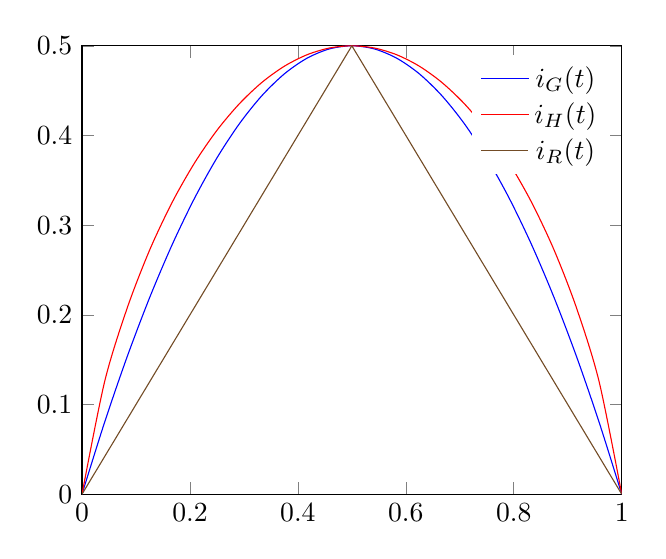
\begin{tikzpicture}
    \begin{axis}[domain=0:1, ymin=0, ymax = 0.5, enlargelimits = false, legend style={draw=none},cycle list name=color]
        \addplot+[no markers, smooth] { 2* x * (1-x) };
        \addlegendentry{$i_G (t)$}
        \addplot+[no markers, smooth] { 1/2*(- x * log2(x) - (1-x)*log2(1-x)) };
        \addlegendentry{$i_H (t)$}
        \addplot+[no markers] { 1 - max(x,1-x) };
        \addlegendentry{$i_R (t)$}
    \end{axis}
    \end{tikzpicture}
    \caption{Comparaison de $i_R$, $i_H$ et $i_G$}
\end{figure}

$i_H$ et $i_R$ répondent toutes les deux aux conditions du théorème~\ref{impurete} mais représentent des quantités différentes. $i_H$ qui est basée sur l'entropie mesure l'incertitude de $Y$ en $t$, avec ce critère d'impureté $\Delta i_H (s,t)$ qu'on appellera alors \emph{gain d'information}. Il représente l'information apprise sur $Y$ en coupant $t$ en $t_L$ et $t_R$. L'impureté de Gini $i_G$ mesure quant à elle avec quelle fréquence un objet $x \in \mathcal{L}_t$ choisi au hasard serait incorrectement classifié s'il était étiqueté par $c \in \mathcal{Y}$ au hasard suivant la loi $p(y \mid t)$. Ces deux notions d'impureté ne sont pourtant pas parfaites, en effet elles présentent toutes les deux la propriété dite \ac{ecp} qui peut rendre un arbre profond et donc difficilement interprétable. De plus les coupes sont biaisées vers la variable possédant le plus de réalisations. De nombreuses alternatives de critères d'impureté existent pour tenter de remédier à ces problèmes telles que le \emph{ratio de gain d'information} utilisé dans les \ac{et}, mais les changements dans la structure de l'arbre induits par le choix de la mesure d'impureté n'ont en réalité que peu d'impact sur la performance en terme de classification \citep{Louppe2014}.

\subsubsection{Régression}

Dans le cas de la régression, c'est-à-dire quand la variable $Y$ est quantitative, il est possible de tout simplement choisir l'erreur $L^2$ locale sans rencontrer les problèmes du cas de la classification.

\begin{definition}
    En régression, la mesure d'impureté $i_R (t)$ issue de l'estimation locale de l'erreur $L^2$ est définie par:
    \begin{equation*}
        i_R (t) = \frac{1}{N_t} \sum_{x,y \in \mathcal{L}_t} (y-\hat{y}_t)^2
    \end{equation*}
\end{definition}
Cela revient donc à minimiser la variance de chacun des noeuds. Il est intéressant de remarquer que le problème de classification binaire avec critère de Gini est en réalité strictement équivalent à un problème de régression avec erreur $L^2$. En effet puisque $\hat{y}_t = \frac{1}{N_t} \sum_{x,y \in \mathcal{L}_t} y = p(c_2 \mid t) = 1 - p(c_1 \mid t)$ on a:
\begin{align*}
    i_R (t) &= \frac{1}{N_t} \sum_{x,y \in \mathcal{L}_t} (y-\hat{y}_t)^2 \\
            &= \hat{y}_t - 2 \hat{y}_t^2 + \hat{y}_t^2 \\
            &= \hat{y}_t (1 - \hat{y}_t) \\
            &= p(c_2 \mid t) (1-p(c_2 \mid t)) \\
            &= \frac{1}{2} i_G (t)
\end{align*}

\subsection{Sélection du point de coupe}

\subsubsection{Familles $\mathcal{Q}$ de règles de partition}

Comme vu précédemment une coupure $s$ du nœud $t$ est une partition disjointe de $\mathcal{X}_t$ où chaque partie disjointe correspond à l'un des fils de $t$. Dans le cas où $s$ partitionne en deux parties disjointes on appelle $s$ une coupure \emph{binaire} de fils $t_L$ et $t_R$, cependant dans le cas plus général, $s$ peut partitionner $\mathcal{X}_t$ en $N$ avec tout autant de fils.
L'ensemble $S$ de toutes les coupures $s$ est l'ensemble de toutes les partitions disjointes de $\mathcal{X}_t$, qui est de cardinal infini dès que les variables peuvent prendre un nombre infini de valeurs, néanmoins il n'est utile de considérer que les partitions qui engendrent une partition de $\mathcal{L}_t$ de parties non vides. Ainsi dans le cadre de l'apprentissage, le problème de trouver la meilleure coupure $s^*$ de $\mathcal{X}_t$ se résume à trouver la meilleure partition du sous-échantillon d'apprentissage $\mathcal{L}_t$. Si l'on considère que les $N_t$ échantillons d'apprentissage sont distincts, le nombre de partitions de $\mathcal{L}_t$ en $k$ sous-ensembles non vides est donné par \citet{Knuth1992}:
\begin{equation*}
    S(N_t,k) = \frac{1}{k!} \sum_{j=0}^k (-1)^{k-j} \binom{k}{j} k^{N_t}
\end{equation*}
qui vaut $2^{N_t-1}-1$ pour une partition binaire. Il est clair que tester naïvement toutes les coupures possibles et ne garder que la meilleure est impossible. Nous allons donc effectuer des hypothèses limitantes sur $s^*$ c'est-à-dire chercher $s^*$ dans une famille $\mathcal{Q} \subseteq \mathcal{S}$ de coupures possibles qui donne toujours une approximation suffisamment bonne de la partition optimale.
Le choix habituel naturel pour $\mathcal{Q}$ est la famille des coupures binaires définies sur une variable unique et sans sous-ensembles vides:
\begin{equation*}
    \mathcal{Q} = \left\{ s \mid \bigcup_{j=1}^p \mathcal{Q}(X_j) , \mathcal{L}_{t_L} \neq \emptyset, \mathcal{L}_{t_R} \neq \emptyset \right\}
\end{equation*}
\begin{itemize}
    \item Si $X_j$ est une variable ordonnée à valeurs dans $\mathcal{X}_j$ alors l'ensemble des coupures binaires sur $X_j$ est: 
    \begin{equation*}
        \mathcal{Q}(X_j) = \left\{ \left( \left\{ x \mid x_j \leq \nu \right\},\left\{ x \mid x_j \geq \nu \right\} \right)  \mid \nu \in \mathcal{X}_j \right\}
    \end{equation*}
    Il s'agit géométriquement de partitions de $\mathcal{X}$ à l'aide d'hyperplans parallèles aux axes.
    \item Si $X_j$ est une variable catégorielle non ordonnée à valeurs dans $\mathcal{X}_j = \{b_1,\dotsc,b_L\}$\label{ntn:b_l} alors on prend pour $\mathcal{Q}(X_j)$:
    \begin{equation*}
        \mathcal{Q}(X_j) = \left\{ \left( \left\{ x \mid x_j \in \mathcal{B} \right\},\left\{ x \mid x_j \in \overline{\mathcal{B}} \right\} \right)  \mid \mathcal{Q} \subset \{ b_1,\dotsc,b_L \} \} \right\}
    \end{equation*}
\end{itemize}
Notre problème de minimisation de l'\emph{impureté} est alors:
\begin{equation*}
\begin{cases}
    s^* = \operatornamewithlimits{argmax}\limits_{ \substack{s_j^* \\ j=1,\dotsc,p}} \Delta i(s^*_j,t) \\
    s^*_j = \operatornamewithlimits{argmax}\limits_{\substack{s \in \mathcal{Q}(X_j) \\ \mathcal{L}_{t_L},\mathcal{L}_{t_R} \neq \emptyset}} \Delta i(s,t)
\end{cases}
\end{equation*}
Bien que le type de partition donné précédemment soit le plus couramment utilisé et celui adopté par Breiman dans les forêts aléatoires classiques et leurs variantes, on notera qu'il n'est pas nécessaire de se restreindre à des hyperplans parallèles aux axes et alors opter pour des coupures dites obliques. On peut même éventuellement utiliser des surfaces de décision non linéaires ou lever la restriction sur le caractère disjoint de la partition.

\subsubsection{Recherche de la coupure binaire optimale}\label{subsubsec:coupure_binaire}

\todo{Mieux expliquer}

Maintenant que le problème d'optimisation est bien défini, il convient de trouver le point de coupure optimal. Il faut alors faire la distinction entre les variables ordonnées et catégorielles. \citet{Louppe2014} propose un algorithme pour chacun des cas afin de simplifier la recherche du point de coupure optimal dans la majorité des cas.

Dans le cas d'une variable ordonnée, il remarque en effet qu'il est possible de calculer $\Delta i(s_j^{\nu'_{k+1}},t)$ à partir de $\Delta i(s_j^{\nu'_{k}},t)$ où $\{ \nu'_{k} \}$ est la famille des points de coupure potentiels ordonnés que l'on choisit comme étant les réalisations dans le cas où $\mathcal{X}_{j}$ est discret et le point médian entre les réalisations dans le cas où $\mathcal{X}_{j}$ est continue.

Dans le cas d'une variable catégorielle et pour la classification binaire une approche naïve forcerait à évaluer $2^{L-1}-1$ partitions, mais \citet{Breiman1984a} prouvent le théorème suivant permettant de se ramener à $L-1$ partitions:

\begin{theoreme}
\label{partition:categ}
    Quitte à réordonner les $X_j$ tel que:
    \begin{equation*}
        p(c_1 \mid t , X_j = b_{l_1} ) \leq p(c_1 \mid t , X_j = b_{l_2} ) \leq \dots \leq p(c_1 \mid t , X_j = b_{l_L} )
    \end{equation*}
    Si $i(t)$ est tel que dans le théorème~\ref{impurete} alors une des $L-1$ sous-parties $\mathcal{B} = \{b_{l_1},\dotsc,b_{l_h} \} $, $h=1,\dotsc,L-1$ définit une partition binaire de l'échantillon du nœud en:
    \begin{align*}
        &\mathcal{L}^{\mathcal{B}}_{t_L} = \{ (x,y) \mid (x,y) \in \mathcal{L}_{t} ,x_j \in \mathcal{B} \} \\
        &\mathcal{L}^{\mathcal{B}}_{t_R} = \{ (x,y) \mid (x,y) \in \mathcal{L}_{t} ,x_j \in \overbar{\mathcal{B}} \}
    \end{align*}
\end{theoreme}
On traite alors $X_j$ comme une variable ordonnée en remplaçant les $b_l$ par $p(c_1 \mid t , X_j = b_{l})$. Malheureusement le théorème~\ref{partition:categ} ne s'étend pas au cas de la classification multiclasse où la seule solution reste d'évaluer les $2^{L-1}-1$ partitions ou, à défaut, un sous-ensemble aléatoire.

\todo{Algo 3.4}

\subsubsection{Coupures aléatoires et \ac{ecp}}

La recherche du point de coupure aléatoire est très chère et le gain apporté par un choix optimal dépend fortement de la régularité de la fonction que l'on cherche à approcher, des caractéristiques de la fonction d'impureté choisie et des caractéristiques de l'espace d'apprentissage $\mathcal{X}$. Au vu de la difficulté de s'assurer que couper de façon optimale apporte un quelconque gain, il peut sembler judicieux d'économiser du temps de calcul en coupant de manière aléatoire.
Il est possible de réduire l'espace de recherche de deux façons:
\begin{itemize}
    \item En ne considérant qu'un sous-ensemble choisi aléatoirement de variables à considérer. Il s'agit de la méthode \ac{rs} introduite par \citet{Ho1998}
    \item En choisissant parmi un ensemble de points de coupures tirés aléatoirement
\end{itemize}
Ces techniques de randomisation sont d'une grande importance pour la construction des forêts aléatoires comme nous le verrons ensuite, on peut donc donner quelques exemples d'arbres aléatoires

\begin{description}
    \item[\ac{extra}]
    Introduits par \citet{Geurts2006}, ici à chaque nœud $K$ variables sont choisies aléatoirement et $K$ points de coupures sont tirés uniformément parmi l'ensemble des valeurs réalisées de chacune de ces variables, la coupure qui minimise l'impureté est alors choisie.
    \item[\ac{UBPRF}]
    Introduit par \citet{Breiman2001} pour ses caractéristiques théoriques, ici on choisit aléatoirement le nœud à partitionner, puis on choisit aléatoirement la variable de coupure et enfin le point de coupure est choisi aléatoirement parmi les réalisations.
    \item[\ac{pert}]
    Dans cette construction de \citet{Cutler2001} il n'y a plus de critère de réduction de l'impureté; à chaque nœud $2$ individus $x_{1,j}$ et $x_{2,j}$ sont tirés aléatoirement de façon à ce qu'ils soient d'une classe différente, puis une variable de coupure est tirée elle aussi aléatoirement. La dernière étape consiste à tirer uniformément sur $[x_{1,j},x_{2,j}]$ un point de coupure. La procédure de construction de l'arbre s'arrête lorsque tous les nœuds actuels sont purs.
    \item[Arbres uniformément aléatoires] 
    Ici \citet{Ciss2013} tire $\lceil \beta d \rceil$ variables avec remise ($\beta > 0$) puis les points de coupures sont choisis uniformément sur le support de $X_j$. Le critère de maximisation de la réduction d'impureté est ici utilisé comme précédemment.
\end{description}

Comme nous le verrons plus tard ces arbres aléatoires sont importants pour la création de forêts aléatoires et présentent souvent de bonnes performances pratiques en évitant les éventuelles caractéristiques problématiques des données. Néanmoins \citet{Ishwaran2014} montre que, du moins dans certains cas, les coupures aléatoires sont moins bonnes que celles vues précédemment. Commençons tout d'abord par introduire la notion de variable de bruit et de propriété \ac{ecp}.

\begin{definition}
    Si $X$ est la caractéristique à $p$ dimensions et $Y$ la variable à prédire on appelle \emph{variable bruyante} une variable $X_j \subseteq \mathcal{X}$ si la loi conditionnelle de $Y$ sachant $X$ est indépendante de $X_j$. Elle est appelée \emph{variable forte} dans le cas contraire.
\end{definition}

\begin{definition}
    Une règle de coupure a la propriété \ac{ecp} si elle tend à couper aux bords pour les variables bruyantes. C'est-à-dire si $\hat{s}_N$ est le point de coupure optimal parmi les points de coupures possibles $x_1 \leq \dotsc \leq x_N$ alors si $X_j$ est bruyante $\hat{s}_N$ tend vers $x_1$ ou $x_N$.
\end{definition}

La propriété \ac{ecp} a longtemps été considérée comme indésirable, car ayant tendance à provoquer des arbres très profonds, mais selon Ishwaran celle-ci est en réalité bénéfique puisqu’en coupant aux bords pour les variables bruyantes on ne dilue pas l'échantillon pour des coupures inutiles et il sera possible de recouper sur des variables fortes plus profondément dans l'arbre.

On peut de plus calculer le point de coupure optimal en fonction de la fonction à estimer $f$ ($Y = f(x) + \varepsilon$) dans le cadre d'une population de nœuds infinie.

\begin{theoreme}
    Soit $\varphi (s) = \mathbb{P} [Y = 1 \mid X = s]$. Si $\varphi (s)$ est continu sur $t = [a,b]$ et $\mathbb{P}$ admet une densité continue positive sur $t$ alors la coupure $s$ optimale au sens de la réduction de l'impureté de Gini dans le cas de la classification binaire est solution de
    \begin{equation}
        2 \varphi (s) = \int_a^s \varphi (x) \mathbb{P}_{t_L} (\diff x) + \int_s^b \varphi (x) \mathbb{P}_{t_R} (\diff x) , a \leq s \leq b
    \end{equation}
\end{theoreme}

\begin{theoreme}
    Le processus de coupure basé sur l'impureté de Gini a la propriété \ac{ecp}.
\end{theoreme}

%\begin{proof}
    \todo{Gini ECP preuve ?}
%\end{proof}

\subsection{Critère d'arrêt}

Plus un arbre de décision est profond, plus son erreur d'apprentissage est faible, mais l'erreur d'apprentissage ne reflète pas forcément l'erreur de généralisation, c'est-à-dire l'erreur sur un échantillon de taille infinie distribué selon la vraie distribution des individus. En effet, un tel arbre a tendance à surapprendre (\emph{overfitting}) et à capturer le bruit plus que l'information. Il est alors nécessaire de trouver un compromis entre sur et sous-apprentissage et donc entre un arbre trop peu profond (l'extrême étant un arbre de profondeur $1$, aussi appelé \emph{souche de décision}) et un arbre trop profond qui obtiendrait alors des performances parfaites sur l'échantillon d'apprentissage et très mauvaises sur l'échantillon test.

\missingfigure{Tradeoff sur/sous apprentissage}

\begin{figure}[htbp]
    \begin{tikzpicture}
    \begin{axis}[ymin=0, ymax = 0.5, enlargelimits = false, xlabel = {Degrés du polynome}, ylabel = {Taux d'erreur}, legend style={draw=none,legend pos=north west}]
            \addplot[no markers, blue] table [x = "i", y = "train", col sep = comma] {images/sursousapp.csv};
            \addlegendentry{Apprentissage}
            \addplot[no markers] table [x = "i", y = "val", col sep = comma] {images/sursousapp.csv};
            \addlegendentry{Validation}
    \end{axis}
    \end{tikzpicture}
    \caption{Sur-apprentissage dans le problème d'apprentissage de $sin(x)$~\ref{fig:biaisvar}}
\end{figure}

Il est donc nécessaire d'avoir une règle d'arrêt de la procédure de coupe récursive. Notons tout d'abord que la procédure de partition possède deux critères d'arrêt inhérents à la procédure:
\begin{enumerate}
    \item lorsque $\mathcal{L}_t$ est homogène, c'est-à-dire que tous les individus ont la même étiquette
    \item lorsque les variables de tous les individus de $\mathcal{L}_t$ sont identiques
\end{enumerate}
Pour empêcher le sur-apprentissage un certain nombre de critères d'arrêt heuristiques peuvent être ajoutés:
\begin{enumerate}
    \item Fixer une taille $N_{\text{min}}$ de l'échantillon pour la partition.
    \item Fixer une profondeur $d_{\text{max}}$ de l'arbre.
    \item Fixer une réduction $\beta$ minimum de l'impureté.
    \item Fixer une taille $N_{\text{feuille}}$ minimum pour chacun des fils en cas de coupure.
\end{enumerate}

Toutes ces variables forment un jeu d'hyper-paramètres qu'il est possible d'optimiser pour obtenir les performances désirées.

\subsection{Importance des variables}

Bien que le but principal d'un algorithme de classification supervisée soit l'étiquetage de nouveaux individus en fonctions de leurs variables, une question naturelle et très importante dans de nombreux domaines comme la bio-informatique est la question de l'importance des variables. Mesurer l'importance des variables dans l'explication du facteur à prédire fournit ainsi une forme d'explication du mécanisme régissant ce facteur. Les arbres aléatoires sont facilement interprétables et il est donc possible d'établir plusieurs mesures de l'importance des variables.

\subsubsection{Diminution de l'impureté}

L'importance de $X_j$ par diminution de l'impureté dans le cas d'un arbre seul est introduite par \citet{Breiman1984a} comme la diminution totale de l'impureté si l'on effectuait les coupures uniquement sur $X_j$ à chaque nœud en imitant la coupure réelle au mieux possible.
C'est-à-dire
\begin{equation*}
    \operatorname{Imp}(X_j) = \sum_{t \in \varphi} \Delta I(\tilde{s}_t^j,t)
\end{equation*}
ou $\tilde{s}_t^j$ est la coupure suppléante en $t$ sur $X_j$, c'est à dire la coupure qui minimise la distance entre les distributions des classes dans les noeuds fils. On remplace toutes les coupures de l'arbre par leur coupure suppléante sur $X_j$ de façon à minimiser les effets de masquage. En effet une variable peut être importante, mais toujours donner une diminution de l'impureté légèrement inférieure aux autres, cette variable ne sera alors jamais sélectionnée et apparaîtrait comme d'importance nulle.

\todo{Donner une formule explicite. EMD ?}

\subsubsection{Diminution de l'erreur}

Il est également possible de mesurer l'importance d'une variable en mesurant sa contribution à la précision de la prédiction. Pour cela on permute les valeurs des observations de la variable $X_j$ d'intérêt, et l'on mesure la diminution de la précision.
\begin{align*}
    \operatorname{Imp}(X_j) &= \frac{1}{N} \sum_{(x'_i,y_i) \in \pi_j(\mathcal{L})} \mathds{1}_{\varphi(x'_i) \neq y_i} \\
    &- \frac{1}{N} \sum_{(x_i,y_i) \in \mathcal{L}} \mathds{1}_{\varphi(x_i) \neq y_i}
\end{align*}
où $\pi_j(\mathcal{L})$ est $\mathcal{L}$ où l'on a permuté les valeurs de $X_j$.
Si $X_j$ est une variable prédictive alors on s'attend à ce que changer ses valeurs détériore le pouvoir prédictif de la forêt.

\subsubsection{Profondeur minimale}

Dans \citet{Ishwaran2007}, l'auteur introduit la notion de $v$ sous-arbre maximal pour étudier les propriétés théoriques de l'importance des variables par diminution de l'impureté. Un $v$ sous-arbre est un sous-arbre dont la racine définit une coupe selon la variable $v$, il est maximal s’il n'est pas lui même $v$ sous-arbre d'un autre $v$ sous-arbre.
Dans \citet{Ishwaran2010a} les auteurs utilisent cette notion de sous arbre pour définir une nouvelle importance de la variable $v$ comme étant la profondeur minimale des $v$ sous-arbres de l'arbre. Il est alors possible de définir l'équivalent pour les forêts en prenant comme importance pour $v$ la profondeur minimale moyenne des $v$ sous-arbres dans la forêt.

Les variables importantes ayant une plus grande chance d'être retenues parmi les différentes variables considérées aléatoirement, on s'attend à ce que les variables importantes soient tirées tôt, les variables peu importantes n'étant tirées qu'en présence uniquement de variables moins importantes, ce qui devrait se produire peu souvent et donc n'arriver en moyenne que profondément dans l'arbre.

\todo{voir \citet{Ishwaran2010a}}

\subsection{Effeuillage}

Afin d'éviter le sur-apprentissage il est essentiel de limiter la complexité de l'arbre. En effet il est trivial en développant l'arbre jusqu'à avoir des feuilles ne comportant qu'un seul individu d'obtenir une erreur nulle sur l'échantillon d'apprentissage. Pour autant l'erreur sur l'échantillon de test explosera.
On a précédemment introduit des critères d'arrêts qui permettent d'éviter ce sur-apprentissage durant la procédure de création de l'arbre mais il est également possible d'effectuer la réduction de la complexité une fois l'arbre entièrement construit.

On procède alors à un \emph{effeuillage} de l'arbre, c'est à dire la suppression des feuilles considérées comme contribuant au sur-apprentissage.

\begin{remark}{Comparaison de différentes méthodes}
    La procédure d'effeuillage n'est pas nécéssaire dans le cas des forêts aléatoires, nous n'exposerons donc ici que une seule méthode possible afin de donner une idée mais il existe d'autres méthodes possibles. Nous renvoyons à \citet{Mingers1989} pour une comparaison des méthodes d'effeuillage d'arbres de décisions seuls.
\end{remark}

Puisque l'on cherche à trouver un compromis entre erreur et complexité, si l'on considère que le nombre de feuilles reflète la complexité d'un arbre alors \citet{Breiman1984a} propose l'algorithme d'\emph{effeuillage coût-complexité}.
On définit par $\left( \varphi_m \right)$ l'ensemble des sous-arbres de $\varphi$, ou un sous-arbre est un arbre obtenu par effeuillage successif de $\varphi$. On cherche alors:
\begin{equation*}
    \argmin_{\varphi_m} \frac{\mathrm{Err} \left[ \varphi_m , \mathcal{L}' \right] - \mathrm{Err} \left[ \varphi , \mathcal{L}' \right] }{\vert \varphi_m \vert_F - \vert \varphi \vert_F}
\end{equation*}
avec $\mathcal{L}'$ un échantillon de test et $\vert \varphi_m \vert_F$ le nombre de feuilles de $\varphi_m$.

\subsection{Consistance}

Bien que de nombreuses variantes des arbres (et par extension forêts) aléatoires sont introduites et étudiées expérimentalement, la théorie permettant d'expliquer les performances est très faible.
Le problème principal est la preuve de la consistance des arbres aléatoires de Breiman.

La consistance des arbres aléatoires est due à \citet{Biau2008,Devroye1997} et se base sur le théorème suivant:

\begin{theoreme}[\citet{Devroye1997}, page 94, théorème 6.1]
    Soit une règle de partionnement telle que:
    \begin{equation*}
        \varphi_n (\mathbf{x}) = \begin{cases}
            0 \text{ si } \sum_{i=1}^n \mathds{1}_{y_i = 1} \mathds{1}_{\mathbf{x}_i \in \mathcal{X}^\varphi (\mathbf{x})} \leq \sum_{i=1}^n \mathds{1}_{y_i = 0} \mathds{1}_{\mathbf{x}_i \in \mathcal{X}^\varphi (\mathbf{x})} \\
            1 \text{ sinon.}
        \end{cases}
    \end{equation*}
    Avec $\mathcal{X} = \bigcup \mathcal{X}^\varphi (x_i)$ la partition (finie) de l'espace définie par le classifieur.
    Notons aussi
    \begin{align*}
        N(\mathbf{x}) = \sum_{i=1}^n \mathds{1}_{\mathbf{x}_i \in \mathcal{X}^\varphi (\mathbf{x})}
    \end{align*}
    le nombre de voisins de $x$, et:
    \begin{equation*}
        \mathrm{diam} ( \mathcal{X}^\varphi ) = \sup_{x,y \in \mathcal{X}^\varphi} \Vert x - y \Vert
    \end{equation*}
    Alors $\mathrm{Err}_n ( \varphi_n ) \to  \mathrm{Err} ( \varphi_B ) $ si 
    \begin{align*}
        &\mathrm{diam} ( \mathcal{X}^\varphi (\mathbf{x}) ) \xrightarrow{\mathbb{P}} 0 \\
        &N ( \mathbf{x} ) \xrightarrow{\mathbb{P}} +\infty
    \end{align*}
\end{theoreme}

\todo{Peut on mettre le theoreme/preuve? Dans le cas Purement aléatoire par exemple???}

\section{Forêts aléatoires}

On a vu dans le chapitre~\ref{chap:trois} comment la création d'ensembles de classifieurs à forte variance permet la construction d'un ensemble de classifieurs de meilleure qualité. Les arbres de classification sont un candidat idéal pour les méthodes ensemblistes grâce à leur capacité à modéliser des relations non linéaires complexes, leurs faibles biais et dans le cas des arbres non effeuillés leur instabilité très élevée. Nous avons également vu qu'il existait plusieurs méthodes pour construire de tels ensembles, néanmoins la plus grande partie des travaux sur les forêts aléatoires porte sur des variantes de la méthode proposée par \citet{Breiman2001}. Nous regrouperons alors toutes ces méthodes sous le terme de Forêts de Breiman.

\begin{remark}{Plus de littérature}
Durant la rédaction de ce rapport un résumé de la littérature sur les forêts aléatoires par \citet{Biau2015} est apparu. Plusieurs autres méthodes sont abordées et les aspects théoriques en particulier font l'objet d'une grande attention. Le rapport technique de \citet{Criminisi2012} porte lui plus sur les aspects pratiques des forêts aléatoires, mais donne un aperçu intéressant des très nombreux problèmes pouvant être résolus par l'apprentissage machine en général et les forêts aléatoires en particulier.
\end{remark}

\subsection{Forêts de Breiman et dérivés}

On a vu dans~\ref{subsec:combinaison_lineaire} que la combinaison linéaire de classifieurs faiblement corrélés permettait la création d'un nouveau classifieur plus puissant. Il est donc nécessaire de construire une famille d'arbres aléatoires les moins corrélés possible avant d'envisager la construction de l'ensemble en lui-même. 

La première façon, dite des \ac{rs}, d'introduire de l'aléa a été introduite par \citet{Ho1998}, elle consiste à chaque étape de création d'une coupure, à tirer aléatoirement un sous-ensemble de $K$ variables de $\mathcal{X}$ puis à appliquer la procédure de choix de la coupe. Le bénéfice de cette technique est double: d'une part en introduisant de l'aléa les arbres sont en partie décorrélés, et d'autre part la réduction du nombre de coupures à considérer accélère grandement la construction de l'arbre.
Néanmoins les arbres restent fortement corrélés et pour pallier ce problème \citet{Breiman1996} introduit le \ac{bagging}. Un échantillon bootstrap de l'échantillon d'apprentissage est tiré avec remise et l'arbre est construit sur ce nouvel échantillon tiré aléatoirement. Ici encore, l'ajout d'aléa permet de décorréler les arbres et de réduire la complexité de construction des arbres d'environ $1/3$ en moyenne. Une autre des propriétés importantes issues de cette technique est l'existence d'un échantillon \ac{oob}. En effet la procédure de tirage avec remise induit qu'en moyenne $1-\left(1-\frac{1}{n}\right)^n \approx 63\% $ des observations sont utilisées pour construire chaque arbre, il est donc possible de mesurer l'erreur \ac{oob} comme approximation de l'erreur de généralisation.

\begin{definition}[Erreur \ac{oob}]
    On appelle erreur \ac{oob}:
    \begin{equation*}
        \hat{\operatorname{Err}}^{\text{OOB}} ( \psi_{\mathcal{L}} ) = \frac{1}{N} \sum_{(x_i,y_i) \in \mathcal{L}} \left( \frac{1}{M^{-i}} \sum_{l=1}^{M^{-i}} \mathds{1}_{\varphi_{\mathcal{L}^{m_{k_l}}} (x_i) \neq y_i} \right)
    \end{equation*}
    ou $m_{k_1},...,m_{k_{M^{-i}}}$ sont les $M^{-i}$ arbres construits à partir d'échantillons bootstrap ne contenant pas $(x_i,y_i)$
\end{definition}

Cette approximation de l'erreur de généralisation est au moins aussi bonne que celle obtenue par $k$-validation croisée \citep{Wolpert1999} tout en étant bien moins coûteuse numériquement.

La version de Breiman possède un bon compromis entre biais et variance et a montré de façon empirique d'excellents résultats sur un grand nombre de problèmes aussi bien artificiels que réels \citep{Fernandez-Delgado2014a}. 

Le caractère guidé, c'est-à-dire la procédure d'optimisation du point du coupe, et le choix de la meilleure coupe parmi $K$ coupes donne aux forêts aléatoires une propriété intéressante qui peut expliquer en partie les très bonnes performances observées, notamment dans le cas des grandes dimensions. En effet \cite{Breiman2004a} montre que la convergence des forêts aléatoires ne dépend que des variables dites \emph{fortes} et non pas les variables \emph{faibles} bruitées. Il montre que la convergence pour une version simplifiée des forêts aléatoires vers l'erreur de Bayes est de l'ordre de
\begin{equation*}
    N^{- \frac{3}{4 \vert S \vert + 3}}
\end{equation*}
avec $S$ les variables fortes définies telles que $\mathbb{E} \left[ y \mid \mathbf{x} \right]$ ne dépend que de $S$. Ce résulat se retrouve pour d'autre types de forêts \citep{Biau2010a} et semble donc se généraliser.

Il existe néanmoins un certain nombre de jeux de données pour lesquels le caractère guidé de l'algorithme \ac{cart} ne présente pas une réduction suffisante du biais, il peut alors être plus efficace de rajouter de l'aléa afin de bénéficier de la réduction de la variance. On peut donc citer deux modifications de l'algorithme de Breiman cherchant à ajouter de l'aléa au détriment du biais.

\begin{figure}[htbp]
    \begin{tikzpicture}
    \begin{axis}[domain=0:1, ymin=0, ymax = 1, enlargelimits = false, xlabel = {Taux de faux positifs}, ylabel = {Taux de vrais positifs}, legend style={draw=none,legend pos=south east}]
            \addplot[no markers, const plot, blue] table [x = "fpr", y = "tpr", col sep = comma] {images/roc_rf.csv};
            \addlegendentry{RF}
            \addplot[no markers, const plot] table [x = "fpr", y = "tpr", col sep = comma] {images/roc_arbre.csv};
            \addlegendentry{Arbre seul}
            \addplot[no markers, const plot, red] table [x = "fpr", y = "tpr", col sep = comma] {images/roc_logreg.csv};
            \addlegendentry{LogReg}
            \addplot[no markers, black, dashed] {x};
    \end{axis}
    \end{tikzpicture}
    \caption{Performances de RF ($\mathrm{AUC} = 0.805$) par rapport à la régression logistique ($\mathrm{AUC} = 0.7889$).}
\end{figure}

\subsubsection{Forêts extrêmement aléatoires}

Cette variante de l'algorithme original introduite dans \citet{Geurts2006} apporte deux modifications lors de la construction des arbres au niveau du critère de sélection et du choix de la coupure.

\begin{description}
    \item[Choix du point de coupe] Ici, le point de coupe de la variable $x_i$ est choisi aléatoirement au lieu de maximiser un critère de réduction d'impureté. Dans le cas ou $x_i$ est numérique on tire un point de coupure aléatoirement sur $ \left[ \min_{\mathcal{L}_t} x_i , \max_{\mathcal{L}_t} x_i \right] $. Dans le cas d'une variable catégorique, on énumère $\mathcal{X}^i_{\mathcal{L}_t}$ le sous-ensemble des valeurs de $x_i$ présentent dans $\mathcal{L}_t$, on tire aléatoirement une sous-partie $\mathcal{X}^i_1 \subset \mathcal{X}^i_{\mathcal{L}_t}$ et $\mathcal{X}^i_2 \subset \mathcal{X}^i \smallsetminus \mathcal{X}^i_{\mathcal{L}_t}$, la coupure choisie est alors $\left( \mathcal{X}^i_1 \cup \mathcal{X}^i_2 , \left(\mathcal{X}^i_1 \cup \mathcal{X}^i_2 \right)^\intercal \right)$.
    \item[Critère de sélection du point de coupe] Ici, l'impureté de Gini est remplacée par le gain d'information, on choisit comme score:
    \begin{equation*}
        \operatorname{Score} (s,\mathcal{L}_t) = \frac{2 I^S_C (\mathcal{L}_t) }{H_S (\mathcal{L}_t) + H_c (\mathcal{L}_t) }
    \end{equation*}
    \todo{Donner les formules des entropies / informations mutuelles}
\end{description}

\begin{figure}[htbp]
    \begin{tikzpicture}
    \begin{axis}[domain=0:1, ymin=0, ymax = 1, enlargelimits = false, xlabel = {Taux de faux positifs}, ylabel = {Taux de vrais positifs}, legend style={draw=none,legend pos=south east}]
            \addplot[no markers, const plot, blue] table [x = "fpr", y = "tpr", col sep = comma] {images/roc_et.csv};
            \addlegendentry{ExtRa}
            \addplot[no markers, const plot] table [x = "fpr", y = "tpr", col sep = comma] {images/roc_rf.csv};
            \addlegendentry{RF}
            \addplot[no markers, black, dashed] {x};
    \end{axis}
    \end{tikzpicture}
    \caption{Performances de ExtRa-Trees ($\mathrm{AUC} = 0.7786$).}
\end{figure}

\subsubsection{Forêts uniformément aléatoires}

Cette variante principalement utile pour ses propriétés théoriques étudiées dans \citet{Ciss2013} présente malgré des hypothèses très restrictives et des simplifications importantes de bonnes performances pratiques de par la forte décorrélation entre les différents arbres. Comme dans le cas des forêts extrêmement aléatoires, les changements dans la construction ont lieu au niveau du choix du point de coupe et du critère de sélection, ainsi que le choix des variables à envisager.

\begin{description}
    \item[Choix des variables de nœuds] On tire à chaque nœud $ \lceil \beta M \rceil $ variables à considérer avec $\beta \in [0,1]$.
    \item[Choix du point de coupe] On tire le point de coupe uniformément sur le support des observations; dans le cas des variables catégorique celles-ci sont converties en variables numériques $1,2,\dotsc,M$.
    \item[Critère de sélection du point de coupe] Le critère à optimiser est ici le \ac{ig} défini par 
    \begin{equation*}
        \operatorname{IG} (Y,X) = \operatorname{H} (y) - \left[ \operatorname{H}(Y \mid X \leq s ) + \operatorname{H}(Y \mid X > s ) \right]
    \end{equation*}
    avec $\operatorname{H}$ l'entropie de Shannon:
    \begin{equation*}
        \operatorname{H} (Y) = \mathbb{E} \left[ -\log \left( \mathbb{P} ( Y = y )  \right) \right]
    \end{equation*}
\end{description}

\begin{figure}[htbp]
    \makebox[\textwidth][c]{
    \begin{tikzpicture}
    \begin{axis}[name= plot1, domain=0:1, ymin=0, ymax = 1, enlargelimits = false, xlabel = {Taux de faux positifs}, ylabel = {Taux de vrais positifs}, legend style={draw=none,legend pos=south east}]
            \addplot[no markers, const plot, blue] table [x = "fpr", y = "tpr", col sep = comma] {images/roc_urf.csv};
            \addlegendentry{URF}
            \addplot[no markers, const plot] table [x = "fpr", y = "tpr", col sep = comma] {images/roc_rf.csv};
            \addlegendentry{RF}
            \addplot[no markers, black, dashed] {x};
    \end{axis}

    \begin{axis}[name = plot2, at=(plot1.right of south east), anchor=left of south west, domain=0:1, ymin=0, ymax = 1, enlargelimits = false, xlabel = {Taux de faux positifs}, legend style={draw=none,legend pos=south east}]
            \addplot[no markers, const plot, blue] table [x = "fpr", y = "tpr", col sep = comma] {images/roc_burf.csv};
            \addlegendentry{BURF}
            \addplot[no markers, const plot] table [x = "fpr", y = "tpr", col sep = comma] {images/roc_rf.csv};
            \addlegendentry{RF}
            \addplot[no markers, black, dashed] {x};
    \end{axis}
    \end{tikzpicture}
    }
    \caption{Performances de URF ($\mathrm{AUC} = 0.8432$) et URF Équilibré ($\mathrm{AUC} = 0.8452$)}
\end{figure}

\subsubsection{Consistance des forêts aléatoires}

La consistance des forêts aléatoires est un problème complexe. La légitimité de leur utilisation n'est pas affectée puisque si l'on fixe un nombre maximal de feuilles, les forêts aléatoires ont une \ac{vc} finie et donc se généralisent bien, mais prouver la convergence vers l'erreur de Bayes ou la convergence vers la vraie distribution dans le cas où l'on estime des probabilités nécessite des techniques particulières.

De nombreux résultats sur la consistance de variantes très aléatoires ou indépendantes des données existent, mais la consistance du classifieur de Breiman n'a été établi que récemment par \citet{Scornet2014a} dans le cas de la régression (on rappelle que la classification binaire peut être vue comme un problème de régression):

\begin{theoreme}[\cite{Scornet2014a}]
    Supposons que:
    \begin{equation*}
        \textbf{(H1)} \quad Y = \sum_{j=1}^p m_j ( x_j ) + \varepsilon
    \end{equation*}
    ou $\mathbf{x} = (x_1, \cdots ,x_p)$ suit une loi uniforme sur $[0, 1]^p$, $\varepsilon \sim \mathcal{N} (0,\sigma^2)$ indépendante et tel que $0 < \sigma^2 < +\infty$, et $m_j$ continus.
    Supposons aussi \textbf{(H2)}:
    Il existe une suite $(\gamma_n)_n \to 0$ telle que $\forall n \in \mathbb{N}^*$ et $1 \leq i$, $j \leq n$ avec $j \neq i$:
    \begin{equation*}
        \left\vert \mathbb{E} \left[ Y_i - \mathbb{E} \left[ Y \mid X = \mathbf{x}_i \right] \mid \mathbf{x}_i,\mathbf{x}_j,y_j,\mathds{1}_{\mathbf{x} \in \mathcal{X}^\varphi (\mathbf{x}_i)},\mathds{1}_{\mathbf{x} \in \mathcal{X}^{\varphi'} (\mathbf{x}_j)} \right]  \right\vert \leq \gamma_n \text{ p.s}
    \end{equation*}
    avec $\varphi'$ une copie identique mais indépendante de $\varphi$ et $\mathds{1}_{\mathbf{x} \in \mathcal{X}^{\varphi} (\mathbf{x}_i)}$ l'indicatrice que $\mathbf{x}$ tombe dans la même feuille que $\mathbf{x}_i$ dans l'arbre $\varphi$.
    Supposons de plus qu'il existe une constante $\sigma'^2 > 0$ telle que $\forall 1 \leq i \leq n$: 
    \begin{equation*}
        \mathbb{E} \left[ \left( Y_i - \mathbb{E} \left[ Y \mid X = \mathbf{x}_i \right] \right)^2 \mid \mathbf{x}_i , \mathds{1}_{\mathbf{x} \in \mathcal{X}^\varphi (\mathbf{x}_i)} \right] \leq \sigma'^2 \text{ p.s}
    \end{equation*}
    Alors sous \textbf{(H1)} et \textbf{(H2)} on a que si:
    \begin{equation*}
        a_n \to +\infty \text{ et } a_n \frac{\log n}{n} \to 0
    \end{equation*}
    avec $a_n$ le nombre d'individus tirés sans remise, alors la forêt aléatoire est consistante.
\end{theoreme}

On retrouve en général dans tous les théorèmes de consistance des forêts aléatoires le même type d'hypothèse pour la consistance:
\begin{equation*}
    k \xrightarrow[n \to +\infty]{} +\infty \text{ et } \frac{k}{n} \xrightarrow[n \to +\infty]{} 0
\end{equation*}
avec $k$ le nombre d'individus dans chaque feuille. Cela se comprend assez bien: on cherche à avoir des feuilles représentant des hypercubes assez petits pour capturer l'ensemble de la distribution tout en ayant assez d'individus dans chaque hypercube pour que l'estimation locale de la probabilité soit elle-même convergente.

\citet{Scornet2014} prouve également que le cas des forêts avec un nombre fini d'arbres présente les mêmes caractéristiques que les forêts infinies ce qui nous permet donc de considérer les forêts aléatoires comme une méthode d'apprentissage statistique avec des garanties théoriques suffisantes pour être valide dans la plupart des cas. (\cite{Biau2008} comporte un contre-exemple de densité atomique dans lequel les forêts ne sont pas consistantes, il faut donc toujours être vigilant.)

\subsection{Forêts obliques}

\subsubsection{Coupes obliques}

Jusqu'à présent, tous les arbres ont utilisé des coupures parallèles aux axes de forme $\{ X_i \leq s \}$, mais il n'est pas obligatoire de se restreindre à des coupures de ce type. Une extension naturelle à ces coupures selon les axes, c'est-à-dire selon un hyperplan formé sur une seule variable, est d'envisager les coupures \emph{obliques} du plan, c'est-à-dire selon des hyperplans reposant sur une combinaison linéaire des variables.

Ainsi il est possible de modifier simplement l'algorithme des forêts classiques pour considérer les coupures multivariées ce qui est l'approche retenue par \citet{Menze2011}. Ici de la même façon que dans la version standard à chaque nœud, seulement $K$ variables sont considérées, mais au lieu de choisir la meilleure coupure sur une seule variable, une coupure oblique sur l'ensemble de ces $K$ variables est considérée. Trois exemples sont considérés dans \citet{Menze2011}:
\begin{description}
    \item[oRF-rnd] Cette version introduite par \citet{Breiman2001} tire $L$ variables au hasard parmi l'ensemble des variables et crée $F$ combinaisons linéaires de coefficients tirés aléatoirement sur $[0,1]$ de celles-ci. La meilleure coupure est sélectionnée parmi les $F$.
    \item[oRF-lda] Ici $K$ variables sont tirées aléatoirement et une surface de décision est créée par \ac{lda}
    \item[oRF-ridge] La surface de décision est créée par régression d'arête (régression linéaire avec régularisation de Tychonoff) sur $K$ variables tirées aléatoirement.
\end{description}

Il est bien sûr possible d'utiliser d'autres algorithmes donnant un hyperplan de séparation, il faut toutefois veiller à la complexité d'un tel algorithme puisque la recherche d'un hyperplan optimal au sens de la mauvaise classification est un problème NP-difficile.

\citet{Barros2011} proposent un algorithme d'induction d'arbres obliques original puisqu'à l'inverse de tous les algorithmes présentés jusque-là, la procédure d'induction de l'arbre commence par les feuilles (\emph{bottom-up}) au lieu de la racine (\emph{top-down}). En commençant l'induction par les feuilles on se libère de la nécessité de posséder une mesure de l'impureté puisque la distribution finale est connue a priori, l'algorithme \emph{BUTIA} donné par les auteurs procède alors de la façon suivante:
\begin{enumerate}
    \item Les individus sont réunis en $K$ ensembles $S_i$ purs avec $K$ le nombre de classe.
    \item $L_i$ clusters sont construits par \ac{em} sur chaque $S_i$ et les centroïdes de chaque cluster sont calculés.
    \item Chaque cluster devient un nœud, les paires des nœuds de centroïdes les plus proches sont fusionnées si elles sont de classes différentes.
    \item Le nouveau nœud se voit attribuer une nouvelle méta classe et un nouveau centroïde et l'hyperplan de séparation optimal est construit par \ac{svm}
    \item Les procédures 1 à 4 sont répétées jusqu'à obtenir la racine.
\end{enumerate}

Bien que les auteurs n'envisagent que le cas de la construction d'un arbre de classification simple, il est toujours possible de construire chaque arbre sur un échantillon boostrap des données et de ne considérer qu'un sous-ensemble $k$ de variables pour la construction des hyperplans à chaque nœud.

\subsubsection{Rotation de l'espace}

L'un des principes de base des forêts de Breiman est la sélection d'un sous-espace de coupure à chaque nœud et nous avons vu précédemment qu'il est possible d'effectuer des coupes obliques comme combinaison linéaire des variables, il est en fait possible de combiner ces deux étapes en une seule et proposer une version plus générale des forêts aléatoires. Cet algorithme introduit par \citet{Tomita2015} utilise des projections de l'espace $\mathcal{X}$ sur un espace de dimension plus petit à chaque étape d'induction de nœuds. Une telle projection possède bien les deux caractéristiques précédentes recherchées: le nouvel espace est de dimension inférieure, une coupe parallèle aux axes dans le nouvel espace est une coupe oblique dans l'espace de base.

Dans l'esprit des forêts aléatoires, afin de garder des arbres faiblement corrélés et donc de bonnes performances de l'ensemble, les projections sont aléatoires. Cette idée est motivée par le théorème de Johnson-Lindenstrauss \citep{Achlioptas2003} selon lequel un petit ensemble de points dans un espace de grande dimension peut être plongé par une projection orthogonale dans un espace de plus petite dimension tout en presque conservant la distance entre les points. C'est à dire:
\begin{lem}[Johnson-Lindenstrauss en distribution]
    $\forall \varepsilon > 0$, $\delta < 1/2$ et $d \in \mathbb{N}^+$ il existe une distribution $\mu$ sur $\mathcal{R}^{k \times d}$ avec $k = O( \varepsilon^{-2} \log ( 1 / \delta) )$ et $A \sim \mu$ tel que:
    \begin{equation*}
        \forall x , \Vert x \Vert = 1 : \mathbb{P} \left( \vert \Vert A x \Vert^2_2 - 1 \vert > \varepsilon \right) < \delta
    \end{equation*}
\end{lem}
Un choix possible pour $A$ qui possède l'avantage d'accélérer grandement le produit matriciel est donné par \citet{Achlioptas2003}:
\begin{equation*}
    A_{i,j} = \sqrt{3} \begin{cases}
        +1 \text{ avec probabilité } 1/6 \\
        0 \text{ avec probabilité } 2/3 \\
        -1 \text{ avec probabilité } 1/6
    \end{cases}
\end{equation*}

Néanmoins les avantages des forêts aléatoires standard étant la robustesse aux données aberrantes et l'invariance aux transformations monotones des variables, il semble naturel de chercher à conserver ces avantages tout en essayant d'obtenir l'invariance par rotation.

Une méthode pour obtenir l'invariance par rotation est la projection \ac{pca} mais celle-ci est coûteuse en temps de calcul. \citet{Tomita2015} proposent donc d'utiliser des Projections Très Creuses \citep{Li2006}: $d$ valeurs dans $\{-1,1\}$ sont tirées avec mêmes probabilités et insérées aléatoirement uniformément dans $A$, la matrice qui en résulte est très creuse, ce qui facilite les calculs, et presque invariante par rotation. Malheureusement, cette projection a pour inconvénient de faire perdre l'invariance par transformation monotone puisque la magnitude relative des variables joue maintenant lorsque celles-ci sont combinées. On peut alors observer que l'algorithme de coupure ne s'intéresse pas aux valeurs en elles-mêmes, mais à leur ordre relatif. Alors avant d'effectuer la projection, la matrice des observations de base est transformée en la matrice des rangs des observations. \todo{en quoi est-ce diffèrent ou mieux que de normaliser ?}
\todo{Mieux expliquer cette partie}
\todo{C'est quoi le principe de Class Conditional Means ????}

\begin{algorithm}
\caption{Randomer Forest} \label{randomer.forest.alg}
\begin{algorithmic}
    \Procedure{Randomer Forest}{$\mathcal{L}, \mu ( \mathcal{L} )$}
    \For{chaque arbre $n$}
        \State{Création du sous-échantillon $\mathcal{L}_n$}
        \For{chaque nœud $i$ de l'arbre}
            \State{$\tilde{X}_{i,n} \gets A^\intercal_{i,n} X_n $ avec $A_{i,n} \sim \mu ( \mathcal{L}_{i,n} ) $}
            \State{$s^*_{i,n} \gets \mathrm{MeilleurCoupure} ( \tilde{X}_{i,n} )$}
            \State{Coupe $\mathcal{L}_{i,n}$ en $\mathcal{L}_{l_i,n}$ et $\mathcal{L}_{r_i,n}$ selon la règle de coupure $s^*_{i,n}$}
        \EndFor
    \EndFor
    \State \Return $\left(\mathrm{Arbres_n},\left( A_{i,n} \right) \right)$
    \EndProcedure
\end{algorithmic}    
\end{algorithm}

\subsection{Forêts bayésiennes}

Nous avons vu dans la partie~\ref{subsec:bma} qu'il était possible de combiner les prévisions d'un ensemble d'arbres dans un modèle bayésien. \citet{Chipman1998} proposent alors une méthode de combinaison bayésienne d'arbres \ac{cart}, mais comme vu en~\ref{subsec:bma}, le \ac{bma} présente certains inconvénients qui impactent les performances de manière négative.
Les auteurs proposent alors \citep{Chipman2008} la construction d'un modèle bayesien sous la forme d'une somme d'arbres, se rapprochant alors de l'esprit du \ac{bmc}.

Les auteurs construisent se placent dans le modèle probit pour la classification. On cherche alors à modéliser
\begin{equation}\label{equ:probleme.probit.bart}
    p(x) \equiv \mathbb{P} \left( Y = 1 \mid x \right) = \Phi ( \varphi(x)  ) 
\end{equation}
où $\Phi$ est la fonction de distribution de la loi normale $\mathcal{N} (0,1)$ et
\begin{equation*}
    \phi (x) = \sum_{i=1}^m \varphi (x,T_i,M_i)
\end{equation*}
Ici $T_i$ est l'arbre $i$, c'est-à-dire l'ensemble des variables et règles de coupures, et $M_i = (\mu_{1i},\dotsc,\mu_{bi})$ le vecteur des étiquettes de ses feuilles et $\varphi$ la fonction de prédiction d'un arbre.

Puisqu'il s'agit d'un modèle bayésien il convient de définir un a priori sur la distribution des arbres. Afin de faciliter les calculs, l'a priori est fixé sous une forme simple:
\begin{equation*}
    \mathbb{P} \left( (T_1,M_1),\dotsc,(T_m,M_m) \right) = \prod_j \left( \mathbb{p}(T_j) \prod_i \mathbb{p}(\mu_{ij} \mid T_j )  \right)
\end{equation*}

\subsubsection{A priori sur $T_i$}

Les auteurs définissent l'a priori $\mathbb{P} ( T_i )$ par:
\begin{description}
    \item $\alpha (1+d)^{-\beta}$ la probabilité qu'un nœud soit terminal.
    \item $\mathcal{U}_{V}$, loi uniforme sur les variables, la probabilité de choisir une variable pour la coupure.
    \item $\mathcal{U}_{[\min X_j , \max X_j]}$, loi uniforme sur les réalisations discrètes de $X_j$, la probabilité de tirer une coupure.
\end{description}

Le processus permettant de tirer un arbre est décrit dans~\citet{Chipman1998}. Les auteurs prennent soin de faire en sorte que le processus de Markov résultant soit réversible. Ainsi le processus de transition $q ( T , T' )$ qui à partir d'un arbre $T$ donne un nouvel arbre $T'$ tire l'une des $4$ modifications suivantes:
\begin{description}
    \item[$\mathbb{P} (\text{AJOUTE} ) = 0.25$] Une feuille est tirée uniformément et une coupure est générée aléatoirement selon la loi a priori de coupure.
    \item[$\mathbb{P} (\text{RETIRE} ) = 0.25$] Le père d'une feuille est tiré aléatoirement et ses deux fils supprimés.
    \item[$\mathbb{P} (\text{CHANGE} ) = 0.4$] Un nœud est tiré aléatoirement et une nouvelle règle de coupure lui est attribué.
    \item[$\mathbb{P} (\text{PERMUTE} ) = 0.1$] Un couple père-fils interne est tiré aléatoirement et leurs règles de coupure sont échangées. Si les deux fils avaient la même règle de coupure alors les deux fils ont leurs règles échangées à la fois.
\end{description}

Ayant ainsi défini un a priori sur les arbres et un processus pour générer des arbres il est possible d'utiliser l'algorithme de Metropolis-Hastings~\ref{sec:metropolis.hastings} pour obtenir une suite d'arbres distribuée selon notre a posteriori.

\subsubsection{A priori sur $\mu_{ij} \mid T_j$}

Encore de façon à faciliter les calculs, les auteurs choisissent
\begin{equation*}
    \mu_{ij} \mid T_j \sim \mathcal{N} ( \mu_\mu , \sigma^2_\mu ) 
\end{equation*}
Comme il en découle que l'a priori sur $\mathbb{E} \left[ Y \mid \mathbf{x} \right]$ est $\mathcal{N} ( m \mu_\mu , m \sigma^2_\mu ) $, on choisit $\mu_\mu$ et $\sigma^2_\mu$ tels que:
\begin{align}
    m \mu_\mu - k \sqrt{m} \sigma_\mu &= \Phi ( -3 ) \\
    m \mu_\mu + k \sqrt{m} \sigma_\mu &= \Phi ( 3 )
\end{align}
pour un $k$ au choix.

Le modèle possède ainsi un très grand nombre de paramètres qui rendent une approche naïve impossible, les auteurs exploitent donc la forme particulière du problème pour mettre en place l'algorithme de \emph{Bayesian Backfitting}, introduit dans~\citet{Hastie2000}. Cet algorithme, tout comme celui de Metropolis-Hastings, repose sur la théorie des \ac{mcmc} exposée dans l'annexe~\ref{annexe:mcmc}. Afin de pouvoir appliquer le Bayesian backfitting, qui consiste à construire la somme progressivement sur les résidus. Dans le cas de la classification il n'y a pas de résidus explicites mais l'on peut réécrire le problème~\ref{equ:probleme.probit.bart} en introduisant $n$ variables latentes $Z_i \sim \mathcal{N} ( \varphi(x) )$ i.i.d telles que $Y_i = 1$ si $Z_i > 0$ et $Y_i = 0$ sinon.

En effet:
\begin{align*}
    \mathbb{P} \left( Y_i = 1 \mid x \right) &= \mathbb{P} \left( Z_i > 0 \mid x \right) \\
    &= \mathbb{P} \left( N + \phi(x) > 0 ) \right) \quad \text{avec } N \sim \mathcal{N} (0,1) \\
    &= \mathbb{P} \left( N > -\phi(x) \right) \\
    &= 1 - \Phi \left( - \phi(x) \right) \\
    \text{(par symétrie)} \qquad &= \Phi( \phi(x) )
\end{align*}

On a de plus $Z_i \mid y_i = 1 \sim \max \left\{ \mathcal{N} ( g(x) , 1 ) , 0 \right\}$, et $Z_i \mid y_i = 0 \sim \min \left\{ \mathcal{N} ( g(x) , 1 ) , 0 \right\}$.

Le problème se ramène alors à un problème de régression et il est possible d'effectuer la procédure de \emph{bayesian backfitting} sur les résidus de $Z$.

L'algorithme BART propose à chaque nouvelle étape un arbre obtenu comme modification locale ce qui réduit la capacité de la chaîne à explorer les zones de faible probabilité, la chaîne se concentrant autour des maximums locaux. Il est de plus nécessaire de recalculer les probabilités a priori et les vraisemblances à chaque étape ce qui est très coûteux. Pour tenter de pallier ces problèmes \citet{Lakshminarayanan2015} propose de remplacer l'algorithme de Gibbs / Metropolis-Hastings par une méthode de Monte-Carlo séquentielle, ou filtre particulaire. Cette modification n'est pas étudiée ici, mais pourrait permettre l'utilisation des forêts bayésiennes sur de grandes bases de données.

\begin{figure}[htbp]
    \begin{tikzpicture}
    \begin{axis}[domain=0:1, ymin=0, ymax = 1, enlargelimits = false, xlabel = {Taux de faux positifs}, ylabel = {Taux de vrais positifs}, legend style={draw=none,legend pos=south east}]
            \addplot[no markers, const plot, blue] table [x = "fpr", y = "tpr", col sep = comma] {images/roc_bart.csv};
            \addlegendentry{BART}
            \addplot[no markers, const plot] table [x = "fpr", y = "tpr", col sep = comma] {images/roc_rf.csv};
            \addlegendentry{RF}
            \addplot[no markers, black, dashed] {x};
    \end{axis}
    \end{tikzpicture}
    \caption{Performances de BART ($\mathrm{AUC} = 0.8365$).}
\end{figure}

Notons également que dans l'algorithme BART, on considère la forêt en elle-même comme le processus de génération des données, mais il est également possible de décider d'un processus de génération des données mêmes et la forêt comme une fonction de ce processus. C'est par exemple le point de vue adopté par \citet{Taddy2015}. Ici les auteurs construisent une forêt bayésienne \textquote{classique} comme agrégation d'arbres et non pas comme somme d'arbres. Il ne s'agit donc pas du tout du même modèle et les performances sont inférieures, mais cette formulation leur permet de définir une adaptation de leur algorithme pour les très grands jeux de données.

\todo{finir !}

\subsection{Amélioration globale de l'erreur des forêts d'arbres}

La procédure standard de forêts aléatoires construit tous les arbres indépendamment sans prendre en compte les prédictions des autres arbres. L'algorithme minimise alors une fonction de perte arbre par arbre avant de les combiner alors qu'idéalement la perte serait minimisée sur la forêt entière. 

Une façon de voir la construction d'un arbre aléatoire, et donc d'une forêt aléatoire, est de voir la procédure de construction de l'arbre comme accomplissant deux tâches distinctes:
\begin{enumerate}
    \item L'apprentissage du \textquote{meilleur} partitionnement de l'espace c'est-à-dire l'apprentissage d'une famille d'indicatrices
    \item L'apprentissage du meilleur étiquetage de chacune des feuilles c'est-à-dire l'apprentissage du meilleur coefficient devant chaque indicatrice.
\end{enumerate}

Ainsi la procédure d'induction d'un arbre consiste à trouver une approximation
\begin{equation}
    \hat{f} (x) = \sum_{k=1}^K \beta_k B_k (x)     
\end{equation}
avec $K$ le nombre de feuilles de l'arbre.
De la même façon pour une forêt composée de $N$ arbres
\begin{equation}
    \hat{f} (x) = \frac{1}{N} \sum_{i=1}^N \sum_{k=1}^{K_i} \beta_k B_{i,k} (x)
\end{equation}

La procédure d'induction des arbres de classification fournit à la fois le partitionnement et l'étiquetage, mais il est également possible de séparer les deux étapes d'apprentissage.

Ainsi \citet{Ren2015} proposent d'optimiser de façon globale la perte des forêts en séparant ces deux étapes d'apprentissage. Une fois les arbres construits il est possible de les interpréter comme des vecteurs indicatrices $\varphi : \mathcal{X} -> \mathbb{R}^K$, ainsi $\varphi (x)$ représente la feuille dans laquelle $x$ tombe. Sous cette forme, on peut alors donner l'étiquetage sous la forme $y_i = \omega \varphi (x_i)$, et apprendre l'étiquetage revient à apprendre le vecteur des poids optimal. Soit pour un arbre seul:
\begin{equation*}
    \begin{aligned}
        & \text{minimiser}
        & & \frac{1}{N} \sum_{i=1}^N l(y_i , \hat{y}_i ) \\
        & \text{tel que} 
        & & y_i = \omega \varphi (x_i ) , \forall i \in [1,N]
    \end{aligned}
\end{equation*}

Sous cette forme apprendre les feuilles d'une forêt est alors
\begin{equation*}
    \begin{aligned}
        & \text{minimiser}
        & & \frac{1}{N T} \sum_{i=1}^N \sum_{t=1}^T l(y_i^t , \hat{y}_i ) \\
        & \text{tel que} 
        & & y_i^t = \omega_t \varphi_t (x_i ) , \forall i \in [1,N], \forall t \in [1,T]
    \end{aligned}
\end{equation*}
Mais cette forme ne correspond pas à l'esprit des forêts aléatoires, on minimise ici la moyenne des pertes sur les arbres au lieu de minimiser la perte de la forêt, il est donc judicieux de modifier notre programme d'optimisation. Pour cela, introduisons le vecteur indicatrice de la forêt globale $\Phi (x) = [\varphi_1 (x), \dotsc, \varphi_T (x)]$ et la matrice des poids des feuilles $W = [\omega_1, \dotsc, \omega_T]$. Il est alors possible d'exprimer la prédiction $y$ de la forêt sous la forme $y = W \Phi (x)$. Il est maintenant possible de minimiser la perte globale de la forêt, afin de se ramener à un problème déjà résolu. \citet{Ren2015} donne le problème d'apprentissage des feuilles sous la forme suivante:
\begin{equation} \label{global.refinement}
    \begin{aligned}
        & \text{minimiser}
        & & \frac{1}{2} \Vert W \Vert^2_2 + \frac{C}{N} \sum_{i=1}^N l(y_i , \hat{y}_i ) \\
        & \text{tel que} 
        & & y_i = W \Phi (x_i ) , \forall i \in [1,N]
    \end{aligned}
\end{equation}
La facilité de résolution de~\ref{global.refinement} vient du fait qu'il s'agit exactement d'un problème de \ac{svm} avec régularisation $L^2$ pour éviter l'overfitting, on choisit alors pour la perte $l$ dans le cas de la classification la perte levier (en se ramenant à des classes $\{-1,1\}$)
\begin{equation*}
    l(x,y) = \max ( 0 , 1 - x \cdot y )
\end{equation*}

Une conséquence de l'optimisation globale des feuilles est qu'il devient alors possible, de la même façon qu'avec les arbres seuls, d'effeuiller la forêt de façon globale pour non seulement réduire de façon considérable la taille de la forêt, mais potentiellement en améliorer le pouvoir de généralisation. La procédure d'effeuillage se fait par étapes successives:
\begin{enumerate}
    \item Calcul du vecteur $W$ selon~\ref{global.refinement}
    \item La somme des normes $l^2$ de toutes les feuilles de même père est calculée
    \item Une proportion $\alpha$ des paires les plus petites sont combinées et le vecteur indicatrice est mis à jour
    \item Répéter la procédure jusqu'à atteindre le critère d'arrêt choisi
\end{enumerate}

\begin{figure}[htbp]
    \begin{tikzpicture}
    \begin{axis}[domain=0:1, ymin=0, ymax = 1, enlargelimits = false, xlabel = {Taux de faux positifs}, ylabel = {Taux de vrais positifs}, legend style={draw=none,legend pos=south east}]
            \addplot[no markers, const plot, blue] table [x = "fpr", y = "tpr", col sep = comma] {images/roc_erf.csv};
            \addlegendentry{ERF}
            \addplot[no markers, const plot] table [x = "fpr", y = "tpr", col sep = comma] {images/roc_rf.csv};
            \addlegendentry{RF}
            \addplot[no markers, black, dashed] {x};
    \end{axis}
    \end{tikzpicture}
    \caption{Performances de ERF ($\mathrm{AUC} = 0.7664$).}
\end{figure}

\subsubsection{Apprentissage des feuilles par maximisation de l'\ac{auc}}

\begin{remark}{\ac{auc} et \ac{erm}}
    Nous avons jusqu'à présent, à travers différentes méthodes, cherché à minimiser une perte empirique, souvent l'erreur empirique. Toutes ces approches étaient naturellement justifiées par la théorie de Vapnik. Malheureusement l'\ac{auc} ne peut pas s'écrire comme la moyenne empirique d'une perte sur l'échantillon puisqu'il s'agit d'une statistique de l'ensemble tout entier et non individu par individu. Il est toutefois possible de se ramener au cadre \ac{erm}, nous renvoyons alors le lecteur vers \citet{Clemencon2006}.
\end{remark}


En considérant le problème sous cette forme, on peut également chercher à optimiser les étiquettes des feuilles pour optimiser le critère qui nous intéresse. En effet, là où l'approche précédente cherche à maximiser la marge et réduire l'erreur de classification, il paraît plus intéressant de chercher à maximiser directement notre critère de performance: l'\ac{auc}.

Optimiser l'\ac{auc} présente deux inconvénients majeurs:
\begin{enumerate}
    \item L'\ac{auc} est une statistique globale de la population et non individu par individu. La calculer nécessite un tri coûteux.
    \item L'\ac{auc} n'est pas différentiable et se prête donc mal aux techniques d'optimisation.
\end{enumerate}
Il faut donc non seulement trouver un substitut différentiable, mais aussi un substitut qui permette de faciliter les calculs pour rendre l'optimisation possible. 
Dans \citet{Calders2007}, les auteurs proposent ainsi deux approximations polynomiales permettant non seulement d'obtenir un substitut différentiable, mais aussi de faire apparaître plusieurs statistiques constantes n'ayant pas besoin d'être mises à jour à chaque étape.

Notons $\mathcal{L} = \mathcal{L_0} \cup \mathcal{L_1}$ avec $\mathcal{L_0}$ les individus négatifs et $\mathcal{L_1}$ ceux positifs. On a alors:
\begin{equation*}
    \mathrm{AUC} ( \varphi , \mathcal{L} ) = \frac{\sum_{k_0 \in \mathcal{L_0}} \sum_{k_1 \in \mathcal{L_1}} \mathds{1}_{\varphi(x_0) < \varphi(x_1)} }{\vert \mathcal{L}_0 \vert \vert \mathcal{L}_1 \vert }
\end{equation*}
La première approche consiste donc à approcher $\mathds{1}$ par une fonction polynomiale, néanmoins il est aussi possible de choisir un substitut dérivable en changeant la fonction:
\begin{gather*}
    \mathrm{AUC} ( \varphi , \mathcal{L} ) = \frac{\sum_{k_0 \in \mathcal{L_0}} \sum_{k_1 \in \mathcal{L_1}} \text{sigmoïde}_\beta \left( \varphi(x_1) - \varphi(x_0) \right) }{\vert \mathcal{L}_0 \vert \vert \mathcal{L}_1 \vert } \\
    \text{sigmoïde}_\beta = \frac{1}{1+e^{-\beta x}}
\end{gather*}
Ce substitut coûte plus cher à calculer, mais présente des avantages propres attrayants selon les auteurs puisqu'il mesure d'une certaine façon la marge en donnant un coût aux points très mal classés et reste une bonne approximation puisque $\text{sigmoïde}_\beta (x) \to H(x) $ lorsque $\beta \to \infty$. Les auteurs proposent donc de l'estimer par une fonction polynomiale.
De façon plus générale, on veut donc approcher
\begin{equation*}
    \mathrm{AUC} ( \varphi , \mathcal{L} ) = \frac{\sum_{k_0 \in \mathcal{L_0}} \sum_{k_1 \in \mathcal{L_1}} f \left( \varphi(x_1) - \varphi(x_0) \right) }{\vert \mathcal{L}_0 \vert \vert \mathcal{L}_1 \vert }
\end{equation*}

En effet nous allons voir qu'utiliser une approximation polynomiale facilite grandement les calculs numériques. Soit $P (x) = \sum_{k}^d \lambda_k x^k$ une approximation polynomiale de la fonction $f$ que l'on souhaite approcher (fonction de Heaviside ou sigmoïde). Alors
\begin{align*}
    f\left( \varphi(x_1) - \varphi(x_0)\right) &\simeq \sum_{k=0}^d \lambda_k \left( \varphi(x_1) - \varphi(x_0)\right)^k \\
    &\simeq \sum_{k=0}^d \lambda_k \sum_{l=0}^k \binom{k}{l} \varphi(x_1)^l (- \varphi(x_0) )^{k-l} \\
    &\simeq \sum_{k=0}^d \alpha_{kl} \sum_{l=0}^k \varphi(x_1)^l \varphi(x_0)^{k-l}
\end{align*}
avec $\alpha_{kl} = \lambda_k \binom{k}{l} (-1)^{k-l} $ et donc:
\begin{equation*}
    \mathrm{AUC} ( \varphi , \mathcal{L} ) \simeq \frac{1}{n_0 n_1} \sum_{k=0}^d \alpha_{kl} \sum_{l=0}^k \left( \sum_{x_1 \in \mathcal{L}_1} \varphi(x_1)^l \right) \left( \sum_{x_1 \in \mathcal{L}_1} \varphi(x_0)^{k-l} \right)
\end{equation*}
Suivant les notations des auteurs on note
\begin{equation*}
    s(\varphi, \mathcal{L}) = \sum_{x \in \mathcal{L}} f(x)
\end{equation*}

En se replaçant dans le cadre précédent d'apprentissage des feuilles on peut alors effectuer une descente de gradient par rapport à $\mathbf{W}$, en notant $\mathrm{AUC}_p$ l'approximation polynomiale de $\mathrm{AUC}$
\begin{align*}
    \frac{\partial \mathrm{AUC}_p (\varphi) }{\partial \mathbf{W}_i} &= \frac{1}{n_0 n_1} \sum_{k=0}^d \sum_{l=0}^k \alpha_{kl} \big( l \cdot s( \Phi(x)_i \left( \mathbf{W} \Phi(x) \right)^{l-1} , \mathcal{L}_1) \cdot s( \left( \mathbf{W} \Phi(x) \right)^{k-l} , \mathcal{L}_0) \\
    &+ (k-l) \cdot s(\left( \mathbf{W} \Phi(x) \right)^l , \mathcal{L}_1) \cdot s( \Phi(x)_i \left( \mathbf{W} \Phi(x) \right)^{k-l-1} , \mathcal{L}_0) \big)
\end{align*}

On peut donc maintenant effectuer la descente de gradient $\mathbf{W}' \leftarrow \mathbf{W} + \gamma \mathbf{g}$, avec $\mathbf{g} = \nabla \mathrm{AUC}$. Nous utilisons alors le fait que l'\ac{auc} est indépendant de la norme de $\mathbf{W}$, donc au lieu de chercher $\gamma$ optimal on peut se contenter de chercher $\mathbf{W}' \leftarrow \cos (\alpha) \mathbf{W} + \sin (\alpha) \nabla \mathbf{g}$. Les auteurs proposent alors une méthode astucieuse exploitant cette forme particulière pour éviter les calculs coûteux.
\begin{align*}
    \mathrm{AUC} (\varphi_{\mathbf{W}'}, \mathcal{L}) &= \frac{1}{n_0 n_1} \sum_{k=0}^d \sum_{l=0}^k \alpha_{kl} \left( \sum_{x \in \mathcal{L}_1} \left( \frac{\cos (\alpha)}{A} \mathbf{W} \Phi(x) + \frac{\sin (\alpha)}{A} \mathbf{g} \Phi(x) \right)^l \right) \\
    & \left( \sum_{x \in \mathcal{L}_0} \left( \frac{\cos (\alpha)}{A} \mathbf{W} \Phi(x) + \frac{\sin (\alpha)}{A} \mathbf{g} \Phi(x) \right)^{k-l} \right)
\end{align*}
où $A$ est un coefficient de renormalisation permettant de rester dans la zone de bonne approximation de notre polynôme. En développant les deux sommes de la même façon que précédemment on retrouve une expression en fonction des fonctions $s$ qui peut être calculée en une seule passe.

\subsection{Forêts en ligne}

Jusqu'à présent toutes les méthodes présentées possédaient un point commun: l'algorithme prend tout $\mathcal{L}$ en entrée et fournit un classifieur en sortie. Il se peut que tous les individus ne soient pas observables immédiatement ou que $\mathcal{L}$ soit trop grand pour permettre l'utilisation de l'algorithme. Dans ce cas, il serait alors préférable de pouvoir mettre à jour le classifieur de façon incrémentale au fur et à mesure que l'on observe les individus. Ce type d'algorithme, appelé \emph{online} et se différenciant des algorithmes \emph{batch}, est d'une importance capitale dès lors que l'apprentissage doit se faire en temps réel par exemple ou dans un environnement aux performances restreintes.

Les forêts aléatoires étant largement utilisées pour de nombreux problèmes, il paraît naturel de tenter de les étendre au problème de l'apprentissage en ligne.

Nous n'exposerons pas ici les différentes méthodes existantes et renvoyons par exemple à \citet{Saffari2009} et \citet{Denil2013} qui proposent des modifications légères de l'algorithme de base où un certain nombre de statistiques descriptives de l'arbre et des individus déjà rencontrés sont gardés en mémoire. À chaque nouvel individu, ces statistiques sont mises à jour et la structure de l'arbre adaptée en conséquence. \citet{Lakshminarayanan2014} définissent une distribution sur les arbres construits sur $N+1$ dont la loi conditionnelle par rapport a l'arbre construit sur $N$ individus est explicite. Cela permet donc à chaque nouvelle observation de générer une nouvelle forêt aléatoire.

Ces algorithmes n'ont pas étés implémentés et testés car leurs performances sont toujours au mieux aussi bonne que la version de base. Leur intérêt est néanmoins évident dans le cadre des bases de données massives.